%\documentclass[draft]{agujournal2018}
\documentclass[]{agujournal2018}
\usepackage{apacite}
\usepackage{url}
\usepackage{lineno}
%\linenumbers
\draftfalse
\journalname{Geophysical Research Letters}

%custom packages
\usepackage{amsmath,amssymb,amsfonts,amsthm}
\usepackage{comment}
\usepackage{booktabs}
% custom commands
\newcommand\be{\begin{equation}}
\newcommand\ee{\end{equation}} 
\newcommand\bra{\langle}
\newcommand\ket{\rangle}
\newcommand\om{\omega}
\newcommand\tom{\tilde{\omega}}
\newcommand\tg{\tilde{g}}
\newcommand\tp{\tilde{p}}
\newcommand\tG{\tilde{G}}
\newcommand\El{\mathcal{L}}
%\usepackage{layouts}
%\printinunitsof{in}\prntlen{\textwidth} % check scales in the document


\begin{document}

\title{Back to Einstein: how to include burial in fluvial sediment diffusion models?}

\authors{James K. Pierce \affil{1}and Marwan A. Hassan\affil{1}}
\affiliation{1}{Department of Geography \\University of British Columbia}
\correspondingauthor{James Kevin Pierce}{kpierce@alumni.ubc.ca}

\begin{keypoints}
\item We develop a random-walk model of objects in intermittent transport through an environment with traps.
\item Its solution provides three ranges of diffusion, two of which are anomalous.
\item We apply the model to sediment transport in rivers to clarify the scale-dependence of bedload diffusion.

\end{keypoints}

\begin{abstract}
	

In gravel-bed rivers, sediment grains transport through a sequence of motions and rests.
When grains rest on the surface, they can be buried by material deposited from upstream.
Buried grains are not exposed to the fluid flow, so these grains are immobile for relatively long periods, only becoming mobile once they're uncovered.  
This crucially affects the transport characteristics of sediment.
Despite the importance of sediment burial to diffusion, very few models have accounted for it.
In this letter, we develop a random-walk model to incorporate sediment burial.
The model predicts three ranges of sediment diffusion with distinct characteristics in each range.
We express the crossover times between these ranges in terms of measurable transport parameters, and explain each range in terms of underlying physical processes.
This provides new geophysical understanding of the scale-dependent phenomenon of fluvial sediment transport.
\end{abstract}

\section{Introduction}
% what is problem and why does it matter
Anomalous diffusion has been the topic of intense research lately, since it appears in contexts as diverse and important as the transport of cholesterols through lipid bilayers \citep{Jeon2012,Molina-Garcia2018}, contaminants through soils \citep{Berkowitz2006,Yang2019}, and pollinator insects through ecosystems \citep{Reynolds2009,Vallaeys2017}.
Emerging research in fluvial geomorphology has come to anomalous diffusion as well, since coarse sediment grains transporting through river channels apparently display it \citep{Martin2012,Bradley2017}.
\citet{Einstein1937} developed the first model of fluvial bedload diffusion, which is the spreading apart of grains as they transport downstream.
Diffusion is induced by differences in the transport characteristics of one grain and the next, and it is usually quantified by the time-dependence of the positional variance $\sigma_x^2(t)$ of a population.
When $\sigma_x^2 \propto t$, the diffusion is said to be normal, since this is found in the classic diffusion problems \citep[e.g.][]{Einstein1905,Taylor1920}.
However, many transport phenomena show $\sigma_x^2 \propto t^\gamma$, with $\gamma \neq 1$. This diffusion is said to be anomalous \citep{Sokolov2012}.
If $\gamma>1$, it is said to be super-diffusive; while if $\gamma <1$, it is said to be sub-diffusive \citep{Metzler2000}.

% what do we know about it 
Researchers after Einstein have come to recognize that coarse sediment moving through river channels can show either anomalous or normal diffusion depending on the timescale of observation \citep{Nikora2002}.
This is a significant issue since it implies diffusion models should be scale dependent, and it renders experimental data contingent on their observation timescales.
\citet{Nikora2001a,Nikora2002} first identified three ranges of bedload diffusion from simulations and experimental data, and they termed these local, intermediate, and global ranges in order of increasing scale.
$\sigma_x^2$ scales with time differently in each range, and this scaling can be anomalous or normal.
Their findings are supported by a wide set of contemporary data and numerical simulations that show up to three ranges of bedload diffusion \citep{Martin2012, Bialik2012, Zhang2012, Fan2016, Bradley2017,Wu2019}.
While earlier works have developed models of bedload diffusion, there are contradictions in the literature about the expected diffusion characteristics (super/normal/sub-diffusion) of each range, and no model has been developed, to our knowledge, that derives all three diffusion ranges from process-based concepts of fluvial sediment transport.

% how do we approach it
In this letter, we present a model of bedload diffusion which describes local, intermediate, and global ranges by including the duration of motion and the possibility of trapping due to burial into the classic bedload diffusion model of \citet{Einstein1937}.
Einstein's model has been highly influential in river geophysics and has fostered an entire paradigm of research that leverages and generalizes his stochastic methods \citep[e.g.][]{Hubbell1964, Yano1969, Yang1971, Gordon1972, Nakagawa1976}.
Its essential content is that individual grains move in instantaneous steps interrupted by durations of rest which lie on statistical distributions \citep{Hassan1991}.
It predicts a single range of normal diffusion \citep{Einstein1937, Nakagawa1976}.
Essentially, the Einstein model is a special case of the continuous time random walk (CTRW) \citep{Montroll1965}, originally developed to describe anomalous diffusion of charge carriers in solids.
To include the duration of motion and the burial process we leverage the multi-state generalization of the CTRW developed by \citet{Weiss1976, Weiss1994}.
Our development allows us to derive three ranges of diffusion and the scaling behavior of $\sigma_x^2$ in each range. The model is analytically solvable, and we determine the cross-over times between diffusion ranges.
Several progressive works have discriminated multiple ranges of bedload diffusion due to the duration of motion \citep{Lisle1998} and sediment burial \citep{Wu2019}, and multiple ranges of diffusion have been shown in models of other transport phenomena \cite[e.g.][]{Bena2006, Balakrishnan1988, Flekkøy2017, AaraoReis2014}.
However, we believe our proposed model is the first analytically solvable model of three diffusion ranges.
We present the model in section \ref{sec:model} and solve it in section \ref{sec:solution}.
We use the solution in section \ref{sec:discussion} to directly attribute physical processes to each diffusion range, to discern the crossover times between ranges in terms of empirically measurable transport parameters, and to derive earlier works as limiting cases \citep[e.g.][]{Lisle1998,Wu2019,Einstein1937}.

\section{Bedload diffusion with burial as a multi-state random walk}
\label{sec:model}
We use a three-state random walk where the states are motion, rest, and burial.
We label these as $i=2$ (motion), $i=1$ (rest), and $i=0$ (burial).
Our development of the governing equations for the three-state walk closely mimics \citet{Weiss1994}, and our approach to incorporating the trapping process closely mirrors \citet{Schmidt2007}. 
In our model, residence times in motion and rest states are random variables characterized by exponential distributions and motions are characterized by a constant velocity $v$.
We consider burial to be a permanent condition which has some probability to occur when resting grains are covered by transported sediment.
The probability of burial per unit time (burial rate) is considered constant, so the probability of trapping increases with the time grains spend resting.

% describe meaning of sojourns and g_i/G_i/theta_i
A central concept in our derivation is the idea of a sojourn in the state $i$ \citep{Weiss1994}.
When a grain enters a state $i$ at some time $t_0$ and position $x_0$, then leaves a state at some other time $t_1$ and position $x_1$, we say that the grain has completed a sojourn in the state $i$. The joint probability density for a complete sojourn through the state $i$ of time $T = t_1-t_0$ and displacement $X = x_1-x_0$ is denoted $g_i(X,T).$ Similarly, we can consider incomplete sojourns. If a grain begins a sojourn in the state $i$ at $(t_0,x_0)$ and the sojourn is still on-going, the joint probability density to find the grain at $(x_1,t_1)$ is $G_i(X,T)$. The $g_i$ and $G_i$ can be further decomposed when time and space components of the motion are independent \citep{Weiss1994}.
We refer to $g_i$ and $G_i$ as the complete and incomplete propagators, since they move probability through space-time and are associated respectively with complete and incomplete sojourns.

% discuss two-stage derivation of weiss
Our target is the probability distribution $p(x,t)$ to find a grain at $x,t$ if we know it started at $(x,t)=(0,0)$, i.e., with the initial distribution $p(x,0)=\delta(x)$.
We denote the initial probabilities to be at rest or in motion as $\theta_1$ and $\theta_2$. 
Normalization requires $\theta_1+\theta_2=1$.
Our derivation has two main steps.
First, we introduce and solve for a set of joint probabilities associated with transitions of a grain from one state to another.
Second, we use these quantities to solve for the probabilities that a grain is in state $i$ having position $x$ at time $t$.
Afterward, we sum the these distributions over all states $i$ to derive the joint probability that a grain is in any state at $(x,t)$.

% derive omegas
Now we begin the first stage of the derivation.
Grains at rest may be trapped by burial.
We consider burial to be permanent \citep[e.g.][]{Wu2019}, and we assume resting grains may be buried with constant probability per unit time $\kappa$.
From this assumption, the probability that a grain is not trapped after a time $t$ at rest is given by a survival probability $\Phi_F(t) = e^{-\kappa t}$ ($F$ is for "free"). Likewise, the probability that it is trapped after resting for a time $t$ is the complement $\Phi_T(t) = 1-\Phi_F(t)$ ($T$ is for "trapped").
We introduce $\omega_{1T}(x,t)$, $\omega_{1F}(x,t)$, and $\omega_2(x,t)$ as the joint probabilities to find a grain at $(x,t)$ having just completed a sojourn.
The subscript ${1T}$ denotes the completion of a rest sojourn due to trapping by burial, while $1F$ denotes the completion of a rest sojourn due to motion.
Similarly, the subscript $2$ denotes the completion of a motion sojourn due to the onset of resting.
Using an argument similar to \citet{Weiss1994}, we write integral equations to link the $\omega$'s: 
\begin{alignat}{2}
&\om_{1T}(x,t) &&= \theta_1\Phi_T(t)g_1(x,t) + \int_0^x dx' \int_0^t dt' \om_2(x',t')\Phi_T(t-t')g_1(x-x',t-t')\label{eq:x}\\
&\om_{1F}(x,t) &&= \theta_1\Phi_F(t)g_1(x,t) + \int_0^x dx' \int_0^t dt' \om_2(x',t') \Phi_F(t-t') g_1(x-x',t-t')\\
&\om_2(x,t) &&= \theta_2 g_2(x,t) + \int_0^x dx' \int_0^t dt' \om_{1F}(x',t')g_2(x-x',t-t') \label{eq:y}
\end{alignat}
The first equation can be understood as follows: $\omega_{1T}(x,t)$ describes the probability that a sojourn in the state $1$ ends due to trapping at $(x,t)$. This quantity has two contributions. The first contribution represents the possibility that the grain started at $(x,t)=(0,0)$ in the $i=1$ state (with probability $\theta_1$), propagated a distance $x$ and a time $t$ in the $i=1$ state (with probability $g_1(x,t)$), was trapped (with probability $\Phi_T(t)$), and is now at $(x,t)$. 
The second contribution describes the possibility that the grain was in a motion sojourn which ended at $x',t'$ when it came to rest. From here, it propagated from $x',t'$ to $x,t$ at rest (with probability $g_1(x-x',t-t')$) and was trapped during this sojourn (with probability $\Phi_T(t-t')$).
The other equations can be reasoned similarly; these arguments are analogous to \citet{Weiss1994}.
Once the propagators are specified, we can solve (\ref{eq:x}-\ref{eq:y}) for the $\omega$'s. This completes the first stage of the derivation.

% derive p's
The second stage of our derivation involves the joint probabilities of being in state regardless of whether a sojourn has just completed. These are denoted by  $p_0(x,t)$ (trapped), $p_1(x,t)$ (rest), and $p_2(x,t)$ (motion), and they involve the $\omega$'s for their definition:
\begin{align}
p_0(x,t) &= \int_0^t dt' \omega_{1T}(x,t-t') \label{eq:b}\\
p_1(x,t) &= \theta_1 G_1(x,t) + \int_0^x dx' \int_0^t dt' \omega_2(x',t')G_1(x-x',t-t')\label{eq:a}\\
p_2(x,t) &= \theta_2 G_2(x,t) + \int_0^x dx' \int_0^t dt'  \omega_{1F}(x',t')G_2(x-x',t-t').\label{eq:z}
\end{align}
Equation (\ref{eq:b}) says that grains buried at any $(x,t)$ arrived there due to trapping at $x$ at any time leading up to $t$.
The reasoning in (\ref{eq:a}-\ref{eq:z}) is the same as for (\ref{eq:x}-\ref{eq:y}), except we use the propagators for incomplete sojourns.
These equations can be solved once the propagators are specified and the $\omega$'s are known from (\ref{eq:x}-\ref{eq:y}).
Finally, we form the total probability density for a grain to be found at $(x,t)$ in any state.
This is simply 
\be p(x,t) = p_0(x,t) + p_1(x,t) + p_2(x,t). \label{eq:dist}\ee
This joint density is completely determined once (\ref{eq:x}-\ref{eq:z}) are solved.


\section{Specification of propagators and solution of model}
\label{sec:solution}
% choice of propagators
We consider sojourns in the rest state to occur for an exponentially distributed time interval, given by the distribution $\psi_1(t) = k_1 e^{-k_1t}.$
The probability that a sojourn in this state lasts for at least the time $t$ is then given by $\Psi_1(t) = \int_t^\infty \psi_1(t)dt = e^{-k_1 t}$.
Since resting grains do not move, the probability of finding the grain at its starting position is $1$, while the probability of finding it anywhere else is zero.
Hence the complete propagator for rest sojourns is $g_1(x,t) = \delta(x)\psi_1(t),$ or 
\be g_1(x,t) = \delta(x)k_1e^{-k_1t}.\label{eq:prop1} \ee
Likewise, the incomplete propagator for a rest sojourn is $G_1(x,t) = \delta(x)\Psi_1(t) = \delta(x)e^{-k_1t} = g_1(x,t)/k_1.$
The motion propagators are reasoned similarly.
We consider motions to occur with a constant velocity $v$ and to have an exponentially distributed duration given by $\psi_2(t) = k_2 e^{-k_2t}.$
Since the velocity of motions is deterministic, the probability to find a grain at position $x$ in a motion sojourn is $\delta(x-vt)$, and the complete propagator for motion sojourns is 
\be g_2(x,t) = \delta(x-vt)k_2e^{-k_2t},\label{eq:prop2}\ee
while the incomplete propagator is $G_2(x,t) = g_2(x,t)/k_2$ as before.

% distribution functions and moments in laplace space
Having defined the propagators, we set out to solve (\ref{eq:x}-\ref{eq:z}) and understand bedload diffusion with a finite motion interval and when subject to trapping by burial.
The convolution structure of (\ref{eq:x}-\ref{eq:z}) presents a formidable problem.
Luckily, we have the device of Laplace transforms.
These project integro-differential equations into an alternate space in which convolutions are unraveled \citep[e.g.][]{Arfken1985}.
The double Laplace transform of a joint probability distribution $p(x,t)$ is defined by 
\be \tilde{p}(\eta,s) = \int_0^\infty dx e^{-\eta x}\int_0^\infty dt e^{-st} p(x,t). \label{eq:doubletransform}\ee
The Laplace-transformed moments of $x$ are linked to derivatives of the double-transformed distribution (\ref{eq:doubletransform}) \citep[e.g.][]{Berezhkovskii2002}.
From (\ref{eq:doubletransform}) it's clear that
\be \bra \tilde{x}(s)^k \ket = (-)^k\partial_\eta^k \tilde{p}(\eta,s)\Big|_{\eta=0}.\label{eq:momenttrick}\ee
The operator $\bra \circ \ket$ denotes the ensemble average \citep[e.g.][]{Kittel1958}.
This means we can compute the variance of position as $\sigma_x^2(t) = \bra x^2 \ket - \bra x \ket^2 = \El^{-1} \{\bra\tilde{x}^2 \ket;t\} - \El^{-1} \{\bra\tilde{x} \ket;t\}^2$, where $\El^{-1}$ denotes the inverse Laplace transform \citep[e.g.][]{Arfken1985}. This is a powerful tool, since we can use it to derive the positional variance without integrating the distribution in equation (\ref{eq:dist}).


% solution for case theta_1=1: distribution function
Using the propagators (\ref{eq:prop1}-\ref{eq:prop2}) and this transform calculus, the joint distribution $p(x,t)$ is derived in appendix \ref{sec:appendixA}, while the moments $\bra x \ket$ and $\bra x^2 \ket$ and ultimately the variance of position $\sigma_x^2(t)$ are derived in appendix \ref{sec:appendixB}. With the shorthand notations $\xi = k_2 x/v$, $\tau = k_1(t-x/v)$, and $\Omega = (\kappa+k_1)/k_1$ \citep[c.f.][]{Lisle1998}, the joint distribution is 
\begin{multline}
p(x,t) = \theta_1\mathcal{H}(\xi)\mathcal{H}(\tau)\Big[1-\frac{k_1}{\kappa+k_1}\Big(1-e^{-(\kappa+k_1)t}\Big)\Big]\delta(x) \\ + \frac{1}{v}e^{-\Omega \tau - \xi}\mathcal{H}(\xi)\mathcal{H}(\tau)\Big(\theta_1\Big[k_1\mathcal{I}_0\big(2\sqrt{\xi\tau}\big) + k_2\sqrt{\frac{\tau}{\xi}}\mathcal{I}_1\big(2\sqrt{\xi\tau}\big)\Big] \\ + \theta_2\Big[k_1\delta(\tau) + k_2 \mathcal{I}_0\big(2\sqrt{\xi\tau}\big)+k_1 \sqrt{\frac{\xi}{\tau}}\mathcal{I}_1\big(2\sqrt{\xi\tau}\big)\Big]\Big) \\
+ \frac{1}{v}\frac{\kappa k_2}{\kappa + k_1}e^{-\kappa \xi/(\kappa + k_1)}\mathcal{H}(\xi)\mathcal{H}(\tau)\Big((\theta_1/\Omega)\mathcal{P}_2(\xi/\Omega,\Omega\tau) + \theta_2 \mathcal{P}_1(\xi/\Omega,\Omega\tau)\Big).
\label{eq:pdf}
\end{multline}
$\mathcal{H}$ is the Heaviside step function and we use the convention $\mathcal{H}(0)=1$.
The $\mathcal{I}_\nu$ are modified Bessel functions of the first kind, and the $\mathcal{P}_\mu$ are generalized Marcum Q-functions defined by $\mathcal{P}_\mu(x,y) = \int_0^y e^{-z-x}(z/x)^{(\mu-1)/2}\mathcal{I}_{\mu-1}(2\sqrt{xz})dz $ \citep{Temme1996}. Modified Bessel functions are common in one-dimensional diffusion problems \citep[e.g.][]{Einstein1937,Daly2010}. The Marcum Q-functions are convolutions between modified Bessel functions and decaying exponentials. They were originally devised in relation to radar detection theory \citep{Marcum1960}. 
Conceptually, the Q-functions emerge in our context from the sediment burial process. According to our assumptions, resting grains can become buried in some interval of time with an exponential probability. Meanwhile, the probability that grains are resting follows a modified Bessel distribution \citep[e.g.][]{Einstein1937,Lisle1998}.
As a result, the probability that sediment is resting and becomes buried involves the convolution structure of the Marcum Q-functions.
Consistent with this interpretation, the terms involving these convolutions vanish when as the burial rate is taken to zero $(\kappa \rightarrow 0)$.
The distribution (\ref{eq:pdf}) is depicted in figure \ref{fig:pdfs} alongside simulations generated by a direct method. The simulation method evaluates the cumulative transition probabilities on a small timestep \citep[c.f.][]{Barik2006}. A link to the simulation code (including descriptive comments) is available in the acknowledgments.

% figure showing distribution functon
\begin{figure}
	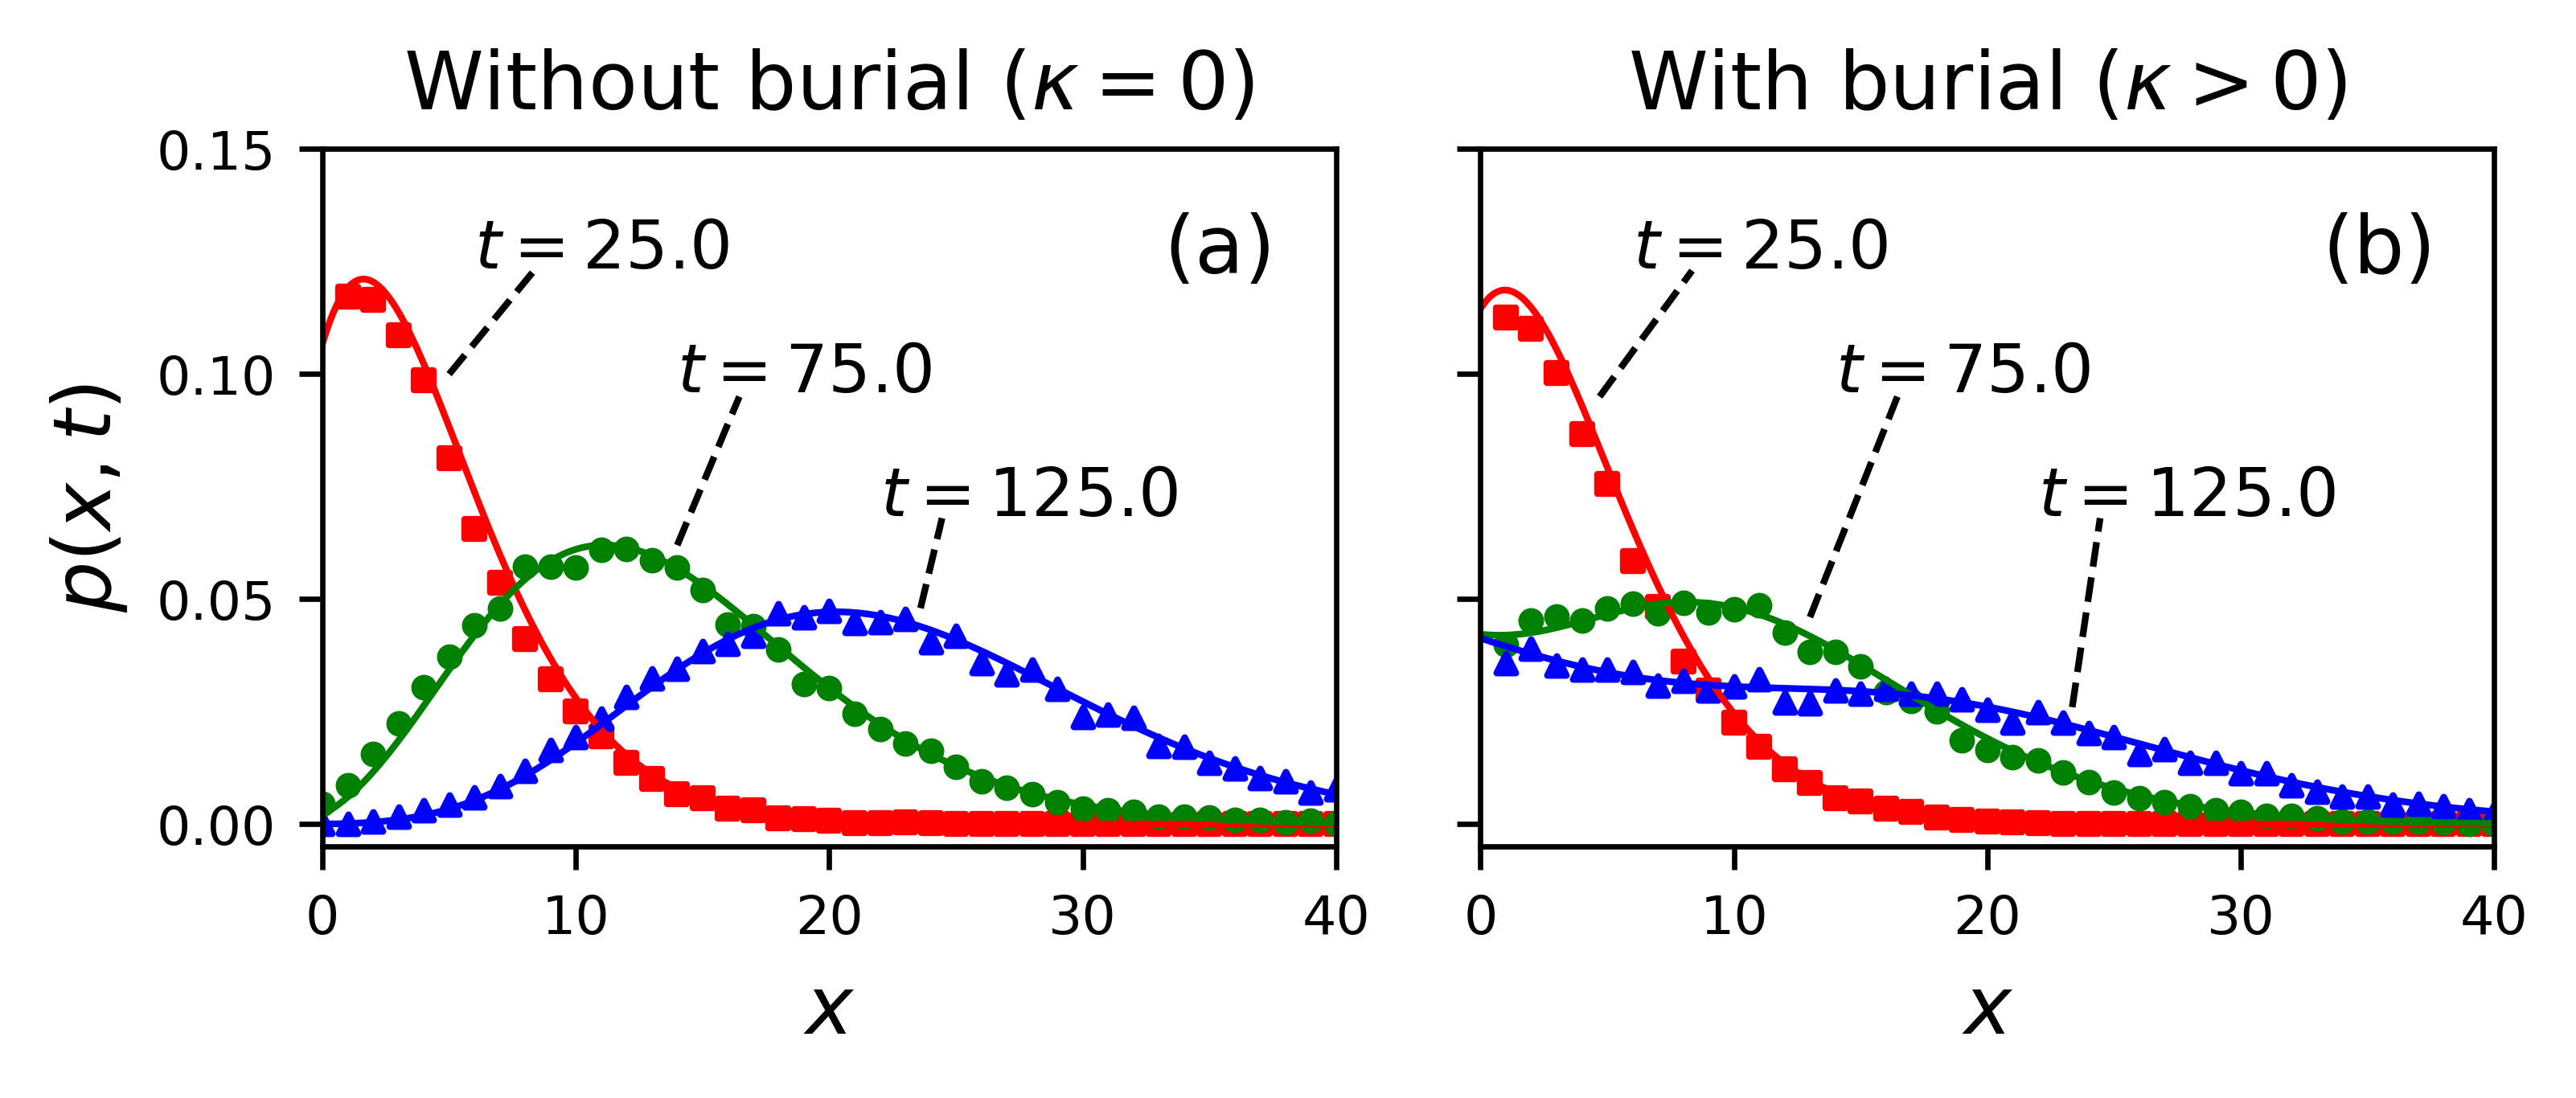
\includegraphics[width=\linewidth,keepaspectratio]{./figures/pdf-plot.png}
	\caption{Joint distributions for a grain to be at position $x$ at time $t$ are displayed for the choice $k_1=0.1$, $k_2=1.0$, $v=2.0$. Grains are considered initially at rest ($\theta_1=1$, $\theta_2=0$). The solid lines are the analytical distribution in equation (\ref{eq:pdf}), while the points are simulation results to show mathematical correctness. Colors pertain to different times. Units are unspecified, since our aim is to demonstrate the general characteristics of $p(x,t)$. Panel (a) shows the case $\kappa=0$ -- the absence of burial.
	In this case, the joint distribution tends toward Gaussian at large times \citep[e.g.][]{Einstein1937,Lisle1998}. Panel (b) shows the case when grains have rate $\kappa = 0.01$ to become buried while resting.
	Because of burial, the joint distribution tends toward a more uniform distribution than Gaussian. This shows a redistribution of probability to smaller values of $x$ due to the burial process \citep[c.f.][]{Wu2019}. The redistribution is encoded mathematically by the Marcum Q-function terms in equation  (\ref{eq:pdf}). A similar tendency is seen in field studies of tracer dispersion in gravel bed rivers \citep[e.g.][]{Hassan1994}.}
	\label{fig:pdfs}
\end{figure}

% solution for theta_1=1: moments
\noindent The first two moments and the positional variance are derived in appendix \ref{sec:appendixB}. 
The moments take the form
\be \bra x(t) \ket = A_1 e^{(b-a)t}+B_1e^{-(a+b)t}+C_1 \label{eq:mean}\ee
\be \bra x^2(t) \ket = A_2(t)e^{(b-a)t}+B_2(t)e^{-(a+b)t}+C_2. \label{eq:second}\ee
In these equations, $a = (\kappa + k_1+k_2)/2$ and $b = \sqrt{a^2-\kappa k_2}$ are effective rates having dimensions of inverse time.
The $A_i$ and $B_i$ are polynomials available in table \ref{table:params}.
The variance is
\be \sigma_x^2(t) = A(t)e^{(b-a)t} + B(t)e^{-(a+b)t} + C(t). \label{eq:var}\ee
$A, B,$ and $C$ are transcendental functions available in table \ref{table:params}.
The positional variance expresses three ranges of diffusion. It is plotted in figure \ref{fig:var}. 
We have made no approximations to derive these results. They are exact, analytical solutions for the transport characteristics of bedload grains transporting downstream as they gradually become buried within the sedimentary bed. More generally, these equations are characteristic of random walkers undergoing diffusion and subjected to permanent trapping while at rest.
\begin{table}[!h]
	\centering
	\caption{Polynomials and transcendental functions used in the expressions of the mean (\ref{eq:mean}), second moment (\ref{eq:second}) and variance (\ref{eq:var}) of bedload tracers.}
	\label{table:params}
	\begin{tabular}{c}
		\toprule
		$\begin{aligned}[t]
		&A_1 = \frac{v}{2b}\big[\theta_2+\frac{k_1+\theta_2\kappa}{b-a}\big] \\
		&B_1 = -\frac{v}{2b}\big[\theta_2-\frac{k_1+\theta_2 \kappa}{a+b}\big] \\
		&C_1 =  -\frac{v}{2b}\big[\frac{k_1+\theta_2 \kappa}{b-a}+\frac{k_1+\theta_2 \kappa}{a+b}\big]\\
		&A_2(t) = \frac{v^2}{2b^3}\Big[(bt-1)[k_1+\theta_2(2\kappa + k_1 + b-a)]+\theta_2b \\
		&\hspace{3cm} + \frac{(\kappa+k_1)(\theta_2\kappa+k_1)}{(b-a)^2}[(bt-1)(b-a)-b]\Big]\\
		&B_2(t) = \frac{v^2}{2b^3}\Big[(bt+1)[k_1 + \theta_2(2\kappa+k_1-a-b)]+\theta_2b\\
		&\hspace{3cm} -\frac{(\kappa+k_1)(\theta_2\kappa+k_1)}{(a+b)^2}[(bt+1)(a+b)+b]\Big]\\
		&C_2 = \frac{v^2}{2b^3}(\kappa+k_1)(\theta_2 \kappa + k_1)\Big[\frac{2a-b}{(b-a)^2}+\frac{a+2b}{(a+b)^2}\Big]\\
		&A(t) = A_2(t)-2A_1C_1 - A_1^2\exp[(b-a)t]\\
		&B(t) = B_2(t)-2B_1C_1 - B_1^2\exp[-(a+b)t]\\
		&C(t) = C_2(t)-C_1^2-2A_1B_1\exp[-2at]\\			
		\end{aligned}$\\
		\bottomrule
	\end{tabular}
\end{table}

\section{Discussion: scale dependence of bedload diffusion}
\label{sec:discussion}

%global range requires further study
\citet{Nikora2002} originally proposed global range sub-diffusion.
\citet{Phillips2013}, \citet{Martin2012}, and \citet{Bradley2010} all probably observed global range super-diffusion, in agreement with our model.
\citet{Weeks1998} analyzed the asymmetric random walk with power law residence times, and found depending on the tail parameter of the resting time distribution and characteristics of the step length distribution, diffusion can be either sub-diffusive or super-diffusive as $t\rightarrow \infty$.
Hence all of these phenomena are conceptually contained in the random walk with power law tails.
\citet{Martin2012, Martin2014, Pierce2019, Bradley2017} have all posited power-law resting time distributions.



\begin{figure}[t]
	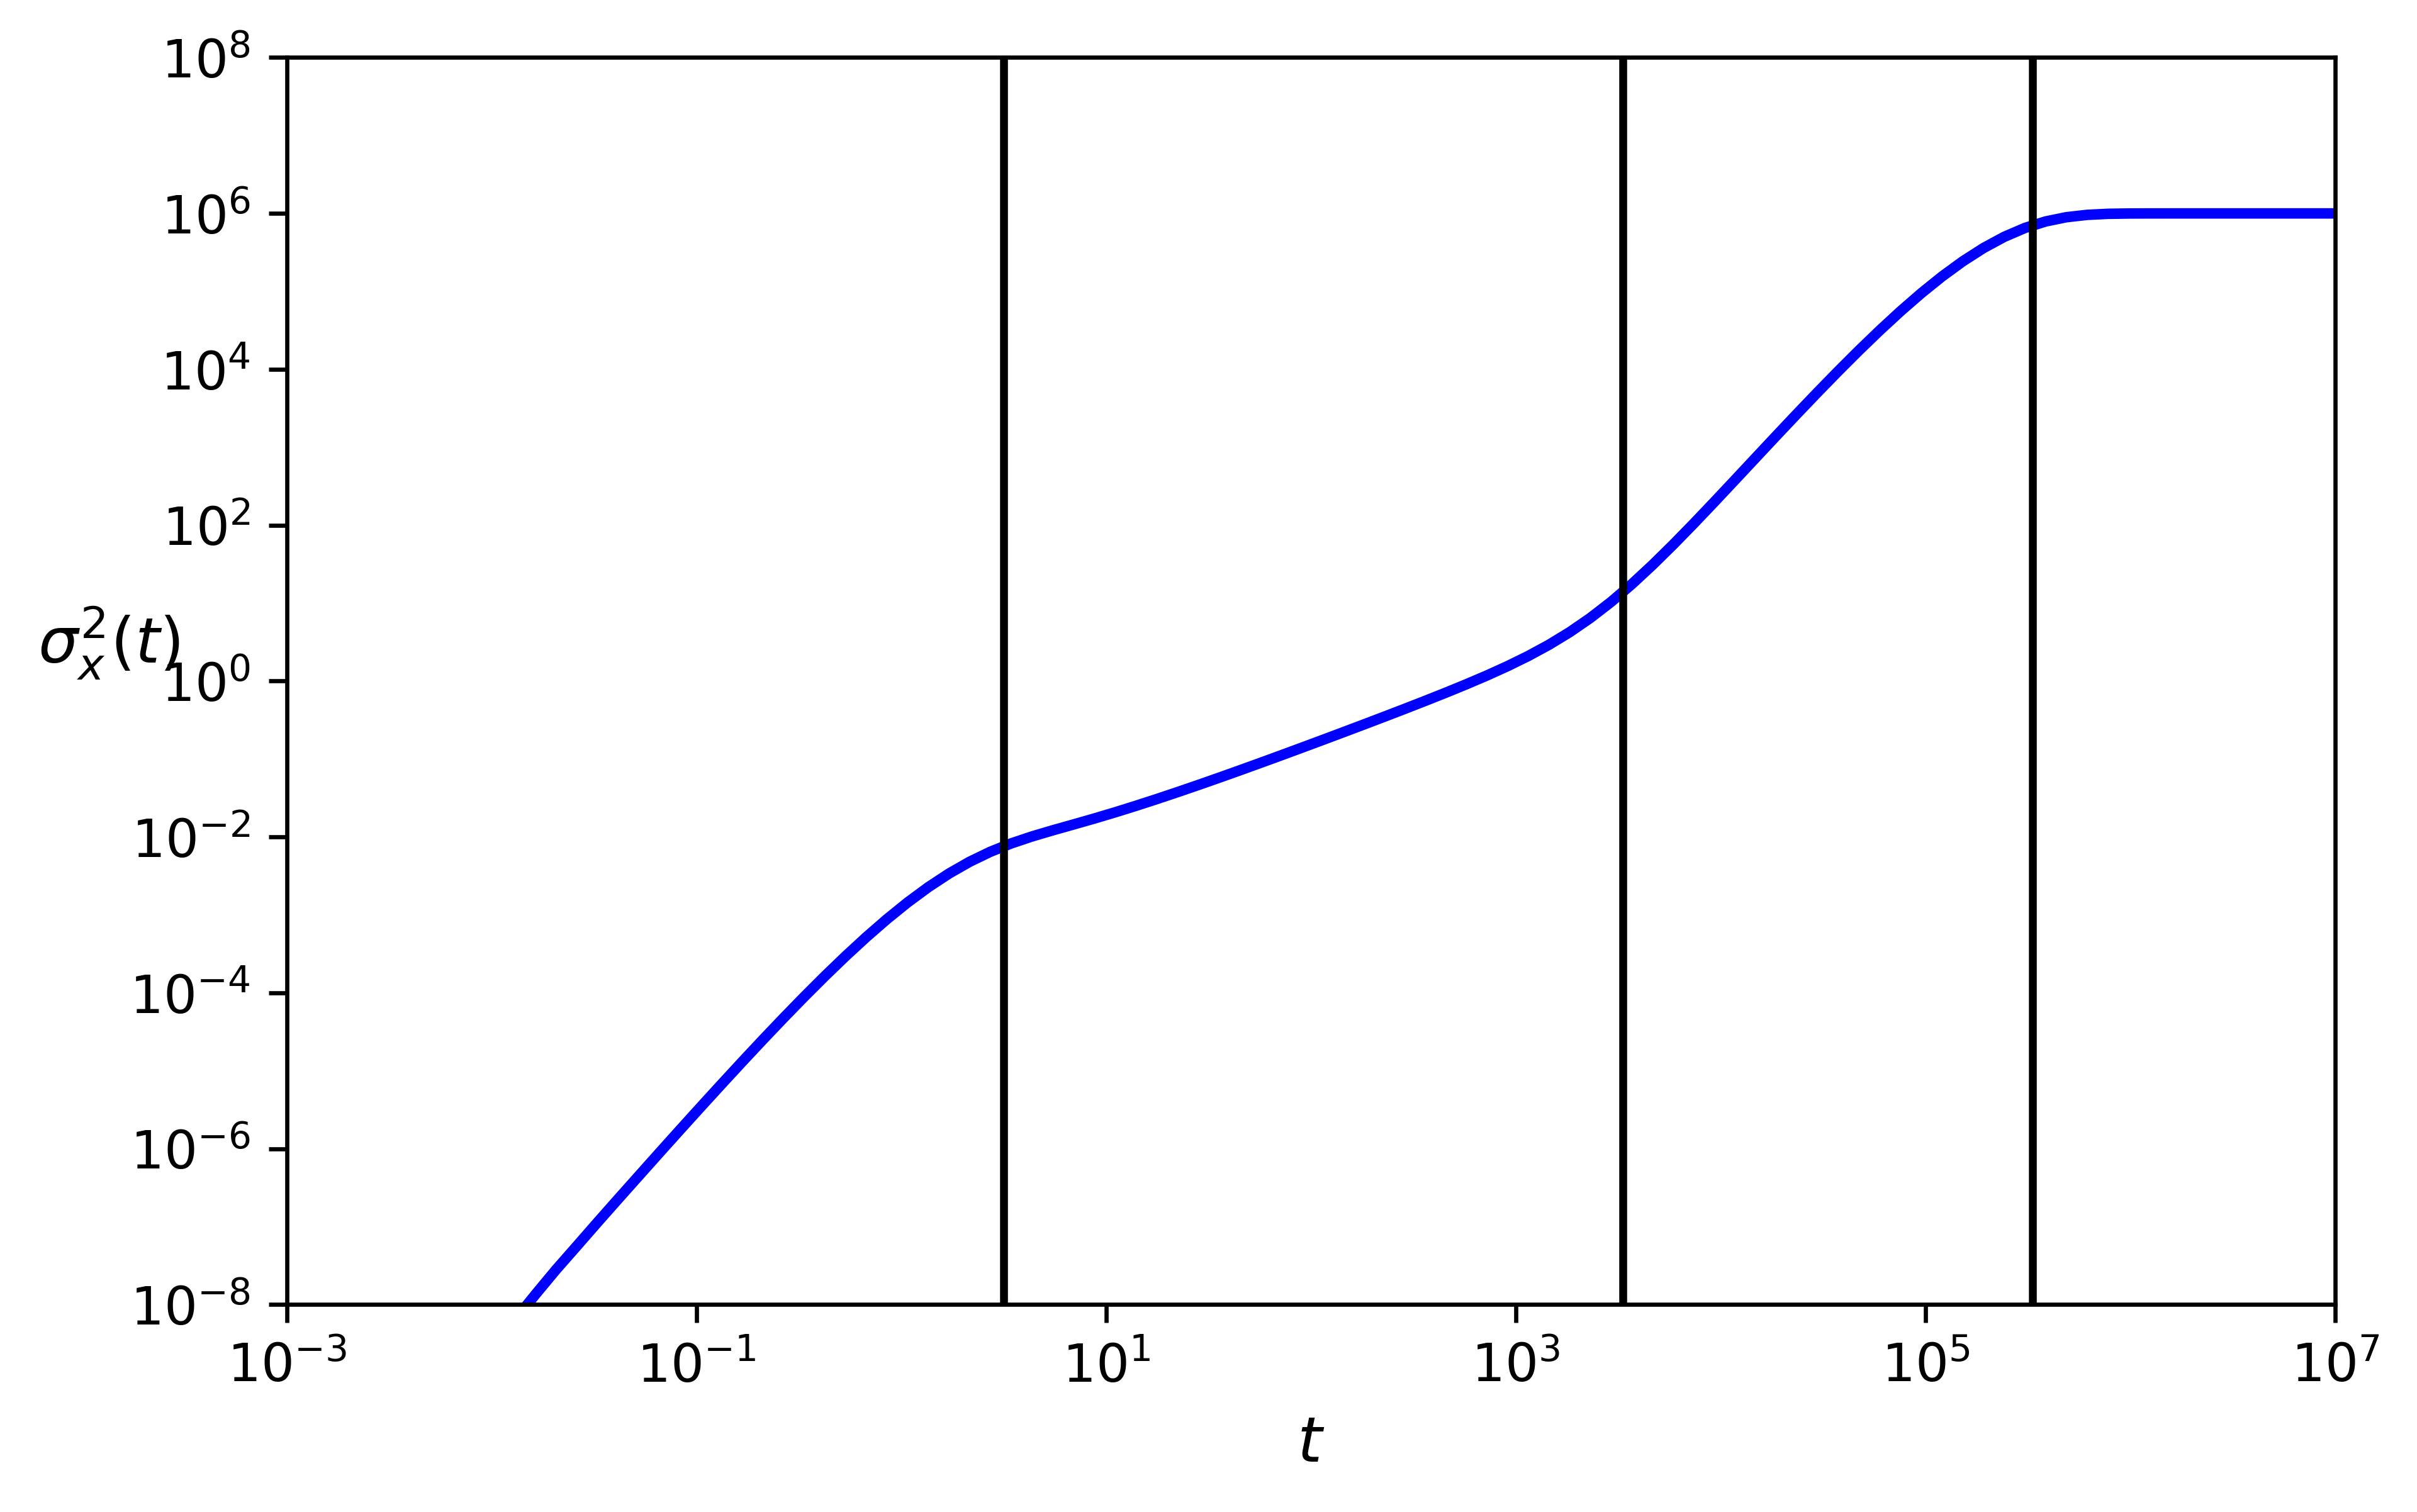
\includegraphics[width=\linewidth,keepaspectratio]{./figures/diffusion.png}
	\caption{Joint distributions to be at position $x$ at time $t$ for parameters $k_1=0.1s^{-1}$,$k_2=1.0s^{-1}$, and $v=2.0ms^{-1}$.}
	\label{fig:var}
\end{figure}

\section{Conclusion}


\appendix

\section{Calculation of the distribution function}
\label{sec:appendixA}
Double transforming (\ref{eq:x}-\ref{eq:y}) using the definition (\ref{eq:doubletransform}) gives
\begin{align}
\tom_{1T}(\eta,s) &= \theta_1 \tg_1(\eta,s) + \tom_2(\eta,s)\tg_1(\eta,s)-\tom_{1F}(\eta,s)\\
\tom_{1F}(\eta,s) &= \theta_1\tg_1(\eta,s+\kappa) + \tom_2(\eta,s)\tg_1(\eta,s+\kappa)\\
\tom_2(\eta,s) &= \theta_2 \tg_2(\eta,s) + \tom_{1F}(\eta,s)\tg_2(\eta,s)
\end{align}
This purely algebraic system solves for 
\begin{align}
\tom_{1T}(\eta,s) &= \frac{\theta_1 + \theta_2 \tg_2(\eta,s)}{1-\tg_1(\eta,s+\kappa)\tg_2(\eta,s)}\big\{\tg_1(\eta,s)-\tg_1(\eta,s+\kappa) \big\} \label{eq:A} \\
\tom_{1F}(\eta,s) &= \frac{\theta_1 + \theta_2 \tg_2(\eta,s)}{1-\tg_1(\eta,s+\kappa)\tg_2(\eta,s)}\tg_1(\eta,s+\kappa)\\
\tom_{2}(\eta,s) &= \frac{\theta_2 + \theta_1 \tg_1(\eta,s+\kappa)}{1-\tg_1(\eta,s+\kappa)\tg_2(\eta,s)}\tg_2(\eta,s). 
\end{align}
Double transforming (\ref{eq:b}-\ref{eq:z}) gives
\begin{align}
\tp_0(\eta,s) &= \frac{1}{s}\tom_{1T}(\eta,s)\\
\tp_1(\eta,s) &= \theta_1 \tG_1(\eta,s) + \tom_2(\eta,s) \tG_1(\eta,s) \\
\tp_2(\eta,s) &= \theta_2 \tG_2(\eta,s) + \tom_{1F}(\eta,s)\tG_2(\eta,s).\label{eq:Z}
\end{align}
The total probability is $p(x,t) = p_0(x,t) + p_1(x,t) + p_2(x,t)$. Using (\ref{eq:A}-\ref{eq:Z}) this becomes, in the double Laplace representation, 
\begin{multline}
\tp(\eta,s) = \frac{1}{s}\frac{\theta_1 + \theta_2 \tg_2(\eta,s)}{1-\tg_1(\eta,s+\kappa)\tg_2(\eta,s)}\big\{\tg_1(\eta,s)-\tg_1(\eta,s+\kappa) \big\} \\
+\frac{\theta_1\big[\tG_1(\eta,s) + \tg_1(\eta,s+\kappa)\tG_2(\eta,s)\big]+ \theta_2\big[\tG_2(\eta,s) + \tg_2(\eta,s)\tG_1(\eta,s)\big]}{1-\tg_1(\eta,s+\kappa)\tg_2(\eta,s)}. \\
\label{eq:lap}
\end{multline}
Using the identities $\tg_i(0,s) = \tilde{\psi}_i(s)$ and $\tG_i(0,s) = (1-\tilde{\psi}_i(s))/s$ \citep[e.g.][]{Weiss1994}, it follows that the joint distribution is normalized in space regardless of the choice of propagators, since $\tp(0,s) = \mathcal{L}\{\int_0^\infty dx p(x,t);s\} = \mathcal{L}\{1;s\} = 1/s$.
Plugging the propagators outlined in equations (\ref{eq:prop1}-\ref{eq:prop2}) into equation (\ref{eq:lap}) gives 
\be \tilde{p}(\eta,s) = \frac{1}{s}\frac{(s+\kappa + k')s  + \theta_1(s+\kappa )\eta v+ \kappa k_2}{(s+\kappa+k_1)\eta v+(s+\kappa+k')s + \kappa k_2}.\label{eq:nicedist}\ee
In this equation, $k'=k_1+k_2$, and we have used the normalization requirement of the initial probabilities $\theta_1 + \theta_2 = 1.$
The double inverse transform of this equation provides the distribution $p(x,t)$.
It is convenient to invert the transform over $\eta$ first.
Using the results 15.103 (transform of exponential), 15.123 (transform of derivative), and 15.141 (transform of Dirac delta function) from \citet{Arfken1985} provides 
\begin{multline} \tp(x,s) = \theta_1 \frac{s+\kappa}{s(s+\kappa + k_1)}\delta(x) + \frac{1}{v} \Big(\frac{(s+\kappa+k')s+\kappa k_2}{s(s+\kappa+k_1)} \\- \frac{\theta_1(s+\kappa)[s(s+\kappa+k_1)+\kappa k_2]}{s(s+\kappa+k_1)^2}\Big)
\exp\Big[-\frac{(s+\kappa+k')s+\kappa k_2}{s+\kappa+k_1}\frac{x}{v}\Big].\end{multline}
Taking the remaining inverse transform over $s$, applying results 15.152 (substitution), 15.164 (translation), and 15.175 (transform of $te^{kt}$) from \citet{Arfken1985}, and defining the shorthand notations $\tau = k_1(t-x/v)$, $\xi = k_2 x/v$, and $\Omega = (\kappa + k_1)/k_1$, gives the simpler form 
\begin{multline}
p(x,t) = \theta_1\Big[1-\frac{k_1}{\kappa + k_1}\big(1-e^{-(\kappa + k_1)t}\big)\Big]\delta(x) + \frac{1}{v}\exp[\Omega \tau - \xi]\\
\times \El^{-1}\Big\{\Big( \theta_2 + \frac{\theta_1k_1+\theta_2 k_2}{s}+\frac{\theta_1k_1k_2}{s^2} + \frac{\theta_2\kappa k_2}{s(s-\kappa-k_1)} + \frac{\theta_1\kappa k_1 k_2}{s^2(s-\kappa-k_1)}\Big)\\
\times\exp\big[\frac{\kappa_1 \xi}{vs}\big];\tau/k_1\Big\}.
\end{multline}
Using entries 2.2.2.1, 2.2.2.8, and 1.1.1.13 from \citet{Prudnikov1992a} in conjunction with the definition of the Marcum Q-function $ \mathcal{P}_\mu(x,t)$ \citep[e.g.][]{Temme1996}, and inserting the Heaviside functions to account for the fact that grains can neither travel backwards nor at speeds exceeding $v$, we finally arrive at equation \ref{eq:pdf} for the joint distribution $p(x,t)$.

\section{Calculation of the moments}
\label{sec:appendixB}
We employ equation \ref{eq:momenttrick} to compute the first two moments of position $x$ and ultimately its variance. The first two derivatives of the double Laplace transformed distribution (\ref{eq:nicedist}) are
\be \partial_\eta \tp(\eta,s) = -v \frac{1}{s}\frac{[(s+\kappa + k')s + \kappa k_2][\theta_2(s+\kappa) + k_1]}{[\eta v(s+\kappa +k_1) + (s+ \kappa + k')s+\kappa k_2]^2},\ee
\be \partial_\eta^2 \tp(\eta,s) = 2v^2 \frac{1}{s} \frac{(s+\kappa+k_1)[(s+\kappa + k')s+\kappa k_2][\theta_2(s+\kappa) + k_1]}{[\eta v(s+\kappa + k_1) + (s+\kappa + k')s+ \kappa k_2]^3}.\ee
Evaluating these at $\eta=0$ and applying equation (\ref{eq:momenttrick}) provides the Laplace transformed moments
\be  \frac{\bra\tilde{x}(s)\ket} {v} = \frac{1}{s}\frac{\theta_2(s+\kappa)+k_1}{(s+\kappa+k')s+\kappa k_2} = \frac{1}{s} \frac{\theta_2(s+\kappa)+k_1}{(s+a+b)(s+a-b)}\label{eq:lapmean},\ee
\be \frac{\bra \tilde{x}^2(s) \ket}{2v^2} = \frac{1}{s} \frac{(s+\kappa+k_1)(\theta_2(s+\kappa)+k_1)}{[(s+\kappa+k')s+\kappa k_2]^2}=  \frac{1}{s}\frac{(s+\kappa+k_1)(\theta_2(s+\kappa)+k_1)}{(s+a+b)^2(s+a-b)^2}.\label{eq:lapsecondmom}\ee
The parameters $a= (\kappa+k')/2$ and $b^2 = a^2 -\kappa k_2$ were introduced to factorize the denominators.
These equations can be inverted using the properties 15.164 (translation), 15.11.1 (integration), and 15.123 (differentiation) from  \citet{Arfken1985} after expansion in partial fractions.
For the mean, the calculation is
\begin{align}
\frac{2b}{v}\bra x \ket &= \big[\theta_2 + (k_1+\theta_2 \kappa)\int_0^t dt\big]\El^{-1}\Big\{ \frac{1}{s+a-b}-\frac{1}{s+a+b};t\Big\}\\
&= \Big[\theta_2 + \frac{k_1+\theta_2\kappa}{b-a}\Big]e^{(b-a)t} - \Big[\theta_2 - \frac{k_1+\theta_2\kappa}{a+b}\Big]e^{-(a+b)t} - \Big[\frac{k_1+\theta_2\kappa}{b-a} + \frac{k_1+\theta_2\kappa}{a+b}\Big].
\end{align}
This equation rearranges to (\ref{eq:mean}).
The second moment (\ref{eq:lapsecondmom}) is 
\begin{multline}
\frac{2b^2}{v^2}\bra x^2 \ket = \Big[\theta_2(\delta(t) + \partial_t) + (\theta_2(2\kappa + k_1)+k_1) + (\kappa+k_1)(\theta_2\kappa+k_1)\int_0^t dt \Big] \\
\times \El^{-1}\Big\{ \frac{1}{(s+a-b)^2} + \frac{1}{(s+a+b)^2}-\frac{1}{b(s+a-b)}+\frac{1}{b(s+a+b)};t\Big\}.
\end{multline}
This becomes 
\begin{multline}
\frac{2b^3}{v^2}\bra x^2 \ket = \Big[\theta_2\partial_t + [\theta_2(2\kappa+k_1)+k_1] + (\kappa+k_1)(\theta_2\kappa+k_1)\int_0^tdt\Big]\\
\times \Big((bt-1)e^{(b-a)t}+(bt+1)e^{-(a+b)t}\Big),
\end{multline}
which evaluates to equation (\ref{eq:second}).
The variance in equation (\ref{eq:var}) results from the algebra $\sigma_x^2 = \bra x^2 \ket - \bra x \ket^2.$

\section{Limiting behavior of the moments}
\label{sec:appendixC}
The easiest approach to extract the earlier results of \cite{Wu2019}, \citet{Lisle1998}, and \citet{Einstein1937} for the moments and positional variance as limiting cases,it's most straightforward to use the Laplace transformed moments (\ref{eq:lapmean}) and (\ref{eq:lapsecondmom}) as a starting point.
An alternate approach is to take limits in the moments (\ref{eq:mean}) and (\ref{eq:second}) directly, but this is somewhat more challenging.
First we obtain the \citet{Wu2019} model as a limit case. 
These authors accounted for sediment burial considering motions to be instantaneous.
They characterized sediment movement by a thin-tailed step length distribution.
This implicitly involves an infinite motion velocity.
To obtain their conclusions on bedload diffusion, we send the mean duration of motion to zero, the velocity to infinity ($1/k_2\rightarrow 0$ and $v\rightarrow \infty$), and we hold the mean step distance $l = v/k_2$ constant.
We use the initial condition that grains start at rest ($\theta_1=1$).
Enacting these limits in equations (\ref{eq:lapmean}) and (\ref{eq:lapsecondmom}) provides
\begin{align}
\bra \tilde{x} \ket &= k_1l\frac{1}{s(s+\kappa)},\\
\bra \tilde{x}^2 \ket &= 2l^2k_1 \frac{s+\kappa+k_1}{s(s+\kappa)^2}.
\end{align}
Inverting these equations and introducing the variables $c=lk_1$ (an effective velocity) and $D_d = l^2k_1$ (a diffusivity) provides positional variance
\be \sigma_x^2(t) = \frac{2D_d(1-e^{-\kappa t})}{\kappa} + \frac{(1-e^{-2\kappa t}-2e^{-\kappa t}\kappa t)c^2}{\kappa^2}.\ee
This is mathematically identical to the key result of \citet{Wu2019}, providing two ranges of diffusion when $\kappa \ll k_1$. One is normal and the other, induced by sediment burial, is super-diffusive.
From here, the \citet{Einstein1937} result can be obtained by turning off the burial process ($\kappa \rightarrow 0$):
\be \sigma_x^2(t) = 2D_d t.\ee
This represents a single range of normal diffusion \citep[c.f.][]{Hubbell1964,Nakagawa1976}.

The \citet{Lisle1998} result can be obtained similarly. For this case, we neglect the burial process $(\kappa \rightarrow 0$) but retain the finite velocity and motion duration in equations (\ref{eq:lapmean}) and (\ref{eq:lapsecondmom}).
For the initial condition $\theta_1=1$, this provides 
\begin{align}
\bra \tilde{x} \ket &= vk_1 \frac{1 }{s^2(s+k')}, \label{eq:li1}\\
\bra \tilde{x}^2 \ket &= 2v^2k_1 \frac{s+k_1}{s^3(s+k')^2}. \label{eq:li2}
\end{align}
Inverting these equations provides the variance of the model when $t\ll 1/\kappa$:
\be \sigma_x^2 = 2v^2k_1\Big(\frac{k_1}{k'^4}\big[\frac{1}{2} - k'te^{-k't} - \frac{1}{2} e^{-2kt}\big] + \frac{k_2}{k'^4}\big[-2+k't + (2+k't)e^{-k't}\big]\Big).\ee
This result encodes two stages of diffusion: at small times there is super-diffusion $\sigma_x^2 \propto t^\gamma$ with $\gamma = 2-3$ depending on the initial condition, and at longer times there is normal diffusion. This links back to the Einstein model in the limit of instantaneous steps: $1/k_2 \rightarrow 0$ and $v\rightarrow \infty$ while $v/k_2 = l$.

Finally, we examine the limit $t\rightarrow 0 $ while leaving $\kappa \neq 0$. This will highlight the effect of initial conditions on the local range super-diffusion of the model we present in this letter.
By applying Tauberian theorems, we can argue the $ t \rightarrow 0$ variance is determined by the $s\rightarrow \infty$ limits of (\ref{eq:lapmean}) and (\ref{eq:lapsecondmom}) \citep[e.g.][]{Weiss1994, Weeks1998}.  Expanding these equations in powers of $1/s \rightarrow 0$ and inverting the resulting transforms gives
\begin{align} \bra x \ket &= v \theta_2 t + \frac{1}{2}v(\theta_1k_1-\theta_2k_2)t^2 + O(t^3),\\
\bra x^2 \ket &= v^2\theta_2 t^2 + \frac{1}{3}v^2(\theta_1k_1-2\theta_2k_2)t^3+ O(t^4).
\end{align}
Taking only leading order terms for each option of $\theta_1$ and $\theta_2$, these equations provide the asymptotic ($t\rightarrow 0$) variance 
\be \sigma_x^2(t) \sim v^2\theta_1\theta_2t^2 + \frac{v^2}{3}[\theta_1k_1+\theta_2k_2]t^3.\ee
In deriving this result, we observe that $t^3$ is the leading order whenever the initial conditions are pure, meaning $\theta_i=0$ for $i=1$ or $i=2$. 
In contrast, when initial conditions are mixed, meaning $\theta_i \neq 0$ for $i=1$ and $i=2$, $t^2$ is the leading order.
This justifies the neglect of factors involving the mixture $\theta_1\theta_2$ in the $O(t^3)$ term. 

\acknowledgments
J. Pierce acknowledges helpful exchanges with Eduardo Daly and Peter H{\"a}nggi during the early stages of this work. He would like to thank Melinda Saunders and Leonardo Golubovic for their careful guidance in mathematics through the years. M. Hassan is supported by an NSERC Discovery grant. The Python simulation code is available at \sloppy
\url{https://github.com/kevinkayaks/rw-diffu}.

\bibliography{biblio.bib}
\end{document}